\newpage
{\color{gray}\hrule}
\begin{center}
\section{Analysis of the Response}
\bigskip
\end{center}
{\color{gray}\hrule}
\begin{multicols}{2}

Following is an analysis that details how the current response of the series $RL$ circuit to the given input wave varies as $R$, $L$, and $\alpha$ change.

\subsection{Case I: $T=\tau$}
\begin{enumerate}
    \item We can note moderate transient effects.
    \item The current tries to reach to its steady-state value each time the voltage is high ($10V$).
    \item When the voltage is low ($0V$), these attempts cease and resume only when the high voltage is achieved again.
    \item As $\alpha$ increases, we can note that the variations in current decrease, owing to the fact that the 'ON' period of the input signal is longer, and thus aids in approaching the steady-state.
\end{enumerate}
All these can be realised in the plot given below: \\
\begin{figure}[H]
  \centering
  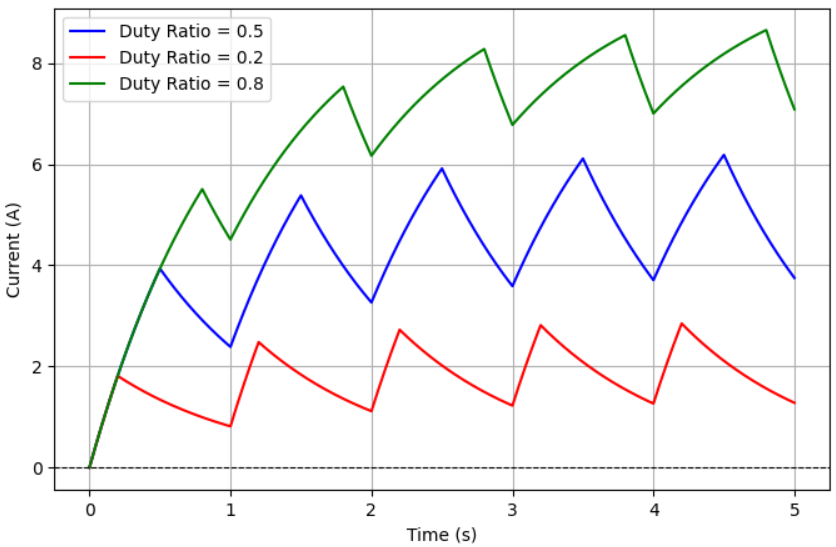
\includegraphics[width=\columnwidth]{sections/6_case1.png}
  \caption{Current Response for $R=1\Omega$, $L=1H$, and $T=1s$}
\end{figure}

\subsection{Case II: $T>\tau$}
\begin{enumerate}
    \item We can note fast transient effects.
    \item The resistor dominates the circuit, and affects its behaviour accordingly.
    \item The current response closely resembles the input voltage wave (regardless of $\alpha$). This is due to the low time constant, which enables the $RL$ circuit to attain steady state current fast.
\end{enumerate}
All these can be realised in the plot given below: \\
\begin{figure}[H]
  \centering
  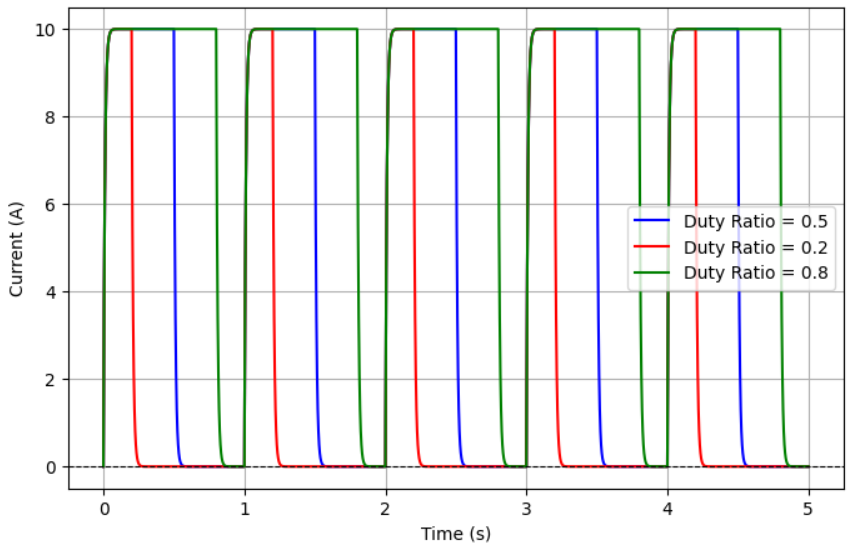
\includegraphics[width=\columnwidth]{sections/6_case2.png}
  \caption{Current Response for $R=1\Omega$, $L=0.01H$, and $T=1s$}
\end{figure}

\subsection{Case III: $T<\tau$}
\begin{enumerate}
    \item We can note a slow transient response.
    \item The inductor dominates the circuit, and affects its behaviour accordingly.
    \item The current struggles to rise at each high voltage ($10V$) due to the inductive nature of the circuit.
    \item As $\alpha$ increases, the current ramps up faster each time the input voltage is high. The current vs. time graph tends to a straight line.
\end{enumerate}
All these can be realised in the plot given below: \\
\begin{figure}[H]
  \centering
  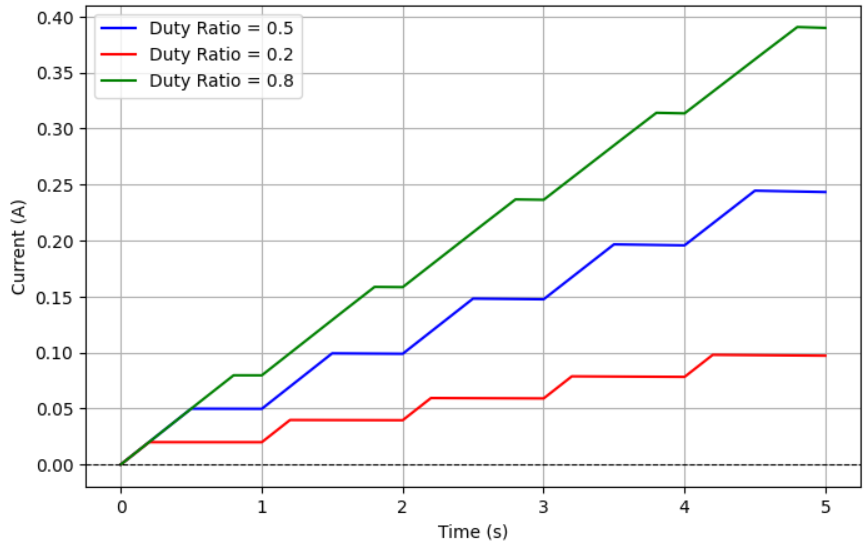
\includegraphics[width=\columnwidth]{sections/6_case3.png}
  \caption{Current Response for $R=1\Omega$, $L=100H$, and $T=1s$}
\end{figure}
\end{multicols}



\newpage
{\color{gray}\hrule}
\begin{center}
\section{Fourier Analysis of Current}
\bigskip
\end{center}
{\color{gray}\hrule}
\begin{multicols}{2}
\subsection{Fourier Transform and Frequency Spectrum}
After calculating the current $I(t)$, we apply the Discrete Fourier Transform (DFT) using the Fast Fourier Transform (FFT) algorithm:
\begin{equation}
I_{\text{FFT}}(k) = \sum_{n=0}^{N-1} I_n e^{-j \frac{2 \pi k n}{N}}
\end{equation}
The magnitude spectrum is computed to analyze the frequency components. The frequency axis is determined as:
\begin{equation}
f_k = \frac{k}{N \Delta t}
\end{equation}
\subsection{Dominant Frequency}
The dominant frequency is the frequency with the highest magnitude in the Fourier spectrum, excluding the DC component at 0 Hz. Ideally, for a square wave with period $T$, the dominant frequency should be:
\begin{equation}
f_{\text{dominant}} \approx \frac{1}{T}
\end{equation}

\subsection{Impact of RL Circuit as Low-Pass Filter}
An RL circuit behaves as a \textbf{low-pass filter}, allowing low-frequency signals to pass while attenuating higher-frequency components. The cutoff frequency is given by:
\begin{equation}
f_c = \frac{R}{2 \pi L}
\end{equation}
For the given parameters:
\begin{equation}
R = 1 \, \Omega, \quad L = 1 \, \text{H} \implies f_c \approx 0.01 \, \text{Hz}
\end{equation}
When the cutoff frequency is much lower than the fundamental frequency of the square wave ($f_{\text{fundamental}} = \frac{1}{T}$), the higher harmonics of the square wave are heavily attenuated. 

\subsection{Why Dominant Frequency is Lower for High-Frequency Input}
When the input square wave has a high frequency, most of its harmonic components lie above the cutoff frequency and are significantly attenuated. As a result, the observed dominant frequency in the current response is much lower than the fundamental frequency of the input square wave:
\begin{equation}
f_{\text{dominant}} \ll \frac{1}{T} \quad \text{when } f_{\text{fundamental}} \gg f_c
\end{equation}

\subsection{Example: High-Frequency Square Wave Attenuation}
Consider an example where:
\begin{itemize}
    \item Period of the square wave: $T = 0.01 \, \text{s} \implies f_{\text{fundamental}} = 100 \, \text{Hz}$
    \item Cutoff frequency of the RL circuit: $f_c \approx 0.01 \, \text{Hz}$
\end{itemize}
Since the square wave's fundamental frequency is much higher than the cutoff frequency, the RL circuit strongly attenuates the harmonics. As a result, the dominant frequency observed in the current is not 100 Hz but a much lower value, approximately equal to the cutoff frequency:
\begin{equation}
f_{\text{dominant}} \approx 0.01 \, \text{Hz}
\end{equation}
This confirms that the RL circuit acts as a low-pass filter, suppressing higher frequencies and causing the dominant frequency to be much lower than expected.
\begin{figure}[H]
  \centering
  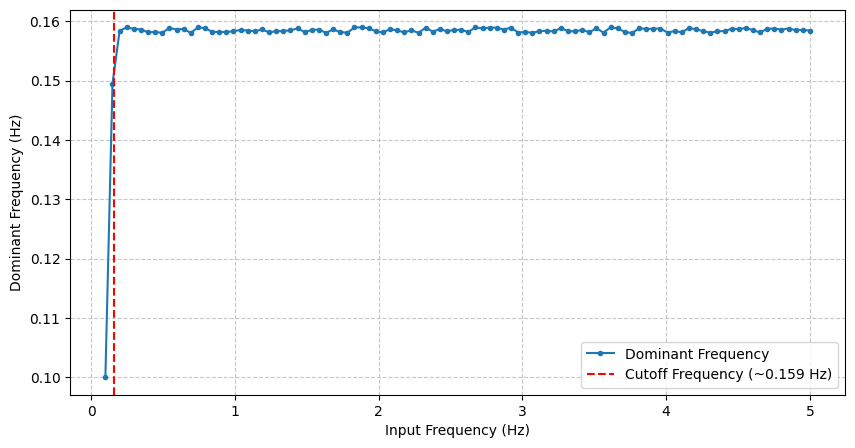
\includegraphics[width=\columnwidth]{sections/dominantfreq.png}
  \caption{Frequency vs Dominant Frequency of $R=1\Omega$, $L=1H$}
\end{figure}
\begin{figure}[H]
  \centering
  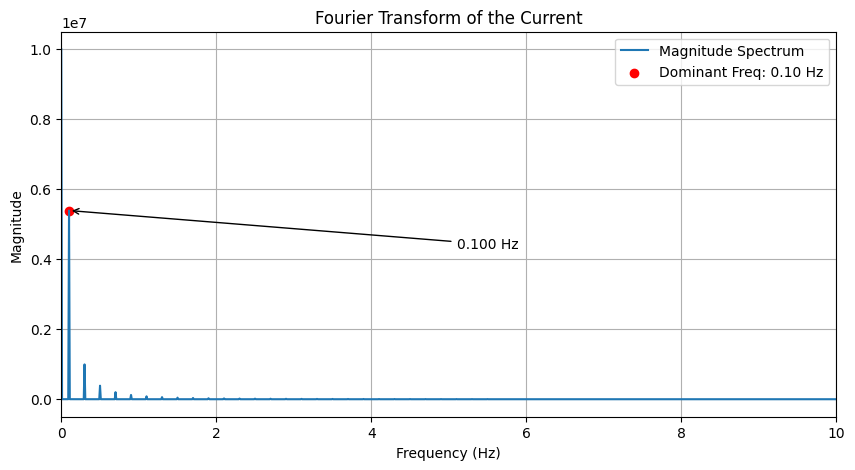
\includegraphics[width=\columnwidth]{sections/fourier_transform.png}
  \caption{Plot of Fourier coefficients of current function when $R=1\Omega$, $L=1H$, and $T=10s$}
\end{figure}
\end{multicols}
